\documentclass[a4paper, 12pt]{article}

\usepackage[portuges]{babel}
\usepackage[utf8]{inputenc}
\usepackage{amsmath}
\usepackage{indentfirst}
\usepackage{graphicx}
\usepackage[colorinlistoftodos]{todonotes}
\usepackage{biblatex} %Imports biblatex package
\addbibresource{refs.bib}
%\bibliography{refs}
\usepackage{siunitx}
\usepackage{float}
\usepackage{amsmath,empheq}
\usepackage{systeme,mathtools}
\usepackage{amsmath}
\usepackage{graphicx,subcaption} 
\usepackage{siunitx}
\usepackage{booktabs}
\usepackage{adjustbox}
\usepackage{array}     % Melhor controle de tabelas
\usepackage{tabularx}  % Tabelas com largura ajustável
\usepackage{amsmath}
% parte para escrever em python
\usepackage[T1]{fontenc}
\usepackage{listings}
\usepackage{listingsutf8}
\usepackage[version=4]{mhchem}
\usepackage[acronym]{glossaries} % habilita glossário de siglas
\makeglossaries
\usepackage{xcolor}
\usepackage{setspace}

\definecolor{codegreen}{rgb}{0,0.6,0}
\definecolor{codegray}{rgb}{0.5,0.5,0.5}
\definecolor{codepurple}{rgb}{0.58,0,0.82}
\definecolor{backcolour}{rgb}{0.95,0.95,0.92}

\lstdefinestyle{mystyle}{
    backgroundcolor=\color{backcolour},   
    commentstyle=\color{codegreen},
    keywordstyle=\color{magenta},
    numberstyle=\tiny\color{codegray},
    stringstyle=\color{codepurple},
    basicstyle=\footnotesize,
    breakatwhitespace=false,         
    breaklines=true,                 
    captionpos=b,                    
    keepspaces=true,                 
    numbers=left,                    
    numbersep=5pt,                  
    showspaces=false,                
    showstringspaces=false,
    showtabs=false,                  
    tabsize=2,
    %literate={á}{{\'a}}1 {ã}{{\~a}}1 {é}{{\'e}}1 {ç}{{\c{c}}}1 {Ç}{{\c{C}}}1
    literate={é}{{\'{e}}}1 {è}{{\`{e}}}1 {ê}{{\^{e}}}1 {ë}{{\¨{e}}}1 {É}{{\'{E}}}1 {Ê}{{\^{E}}}1 {û}{{\^{u}}}1 {ù}{{\`{u}}}1 {â}{{\^{a}}}1 {à}{{\`{a}}}1 {á}{{\'{a}}}1 {ã}{{\~{a}}}1 {Á}{{\'{A}}}1 {Â}{{\^{A}}}1 {Ã}{{\~{A}}}1 {ç}{{\c{c}}}1 {Ç}{{\c{C}}}1 {õ}{{\~{o}}}1 {ó}{{\'{o}}}1 {ô}{{\^{o}}}1 {Õ}{{\~{O}}}1 {Ó}{{\'{O}}}1 {Ô}{{\^{O}}}1 {î}{{\^{i}}}1 {Î}{{\^{I}}}1 {í}{{\'{i}}}1 {Í}{{\~{Í}}}1 {°}{\textdegree}1, 
}
 
\lstset{style=mystyle}


% Note that the sign must be
%  µ
%  MICRO SIGN
%  Unicode: U+00B5, UTF-8: C2 B5
% and \emph{not}
%  μ
%  GREEK SMALL LETTER MU
%  Unicode: U+03BC, UTF-8: CE BC
\sisetup{math-micro=\text{µ},text-micro=µ}

%title{Experiência 3: Máquinas Síncronas}

%author{Caio Rosa \\ João Antônio do Amarante \\ Rodrigo \\ Thuane}

%\date{\today}
\setlength {\marginparwidth }{2cm}
\usepackage{hyperref}
\hypersetup{
    colorlinks=true,
    linkcolor=blue,
    filecolor=magenta,      
    urlcolor=cyan,
    pdftitle={Overleaf Example},
    pdfpagemode=FullScreen,
    }

\urlstyle{same}

\begin{document}
%\maketitle

\begin{titlepage}
	\begin{center}
%		\huge{Universidade de Caxias do Sul}

\vspace{10pt}
\begin{figure}[!ht]
\centering

\includegraphics[width=3.5cm]{logo_ucs.png}
\end{figure}
        
        \vspace{45pt}
        
		\textbf{{\LARGE
                \begin{spacing}{1.2}
            \textbf{Relatório para o módulo de Análise Linear Pelo Método de Elementos Finitos da Especialização em Simulações Estruturais, Fluidodinâmicas e 
Multicorpos: Instrumentação e Durabilidade}
            \end{spacing}}}
		\vspace{70pt}
		
	\end{center}
	
	\begin{flushleft}
		\begin{tabbing}
			Aluno\qquad\qquad\= Antonio Victor de Souza Correa \\
			Professor\> MSc. Alexsandro Sordi\\
			
		
	\end{tabbing}
		  
	\end{flushleft}
	
	\begin{center}
		\vspace{\fill}
		Rio de Janeiro, Outubro de 2026
	\end{center}
\end{titlepage}
%%%%%%%%%%%%%%%%%%%%%%%%%%%%%%%%%%%%%%%%%%%%%%%%%%%%%%%%%%%
\newpage
\tableofcontents
\thispagestyle{empty}

\newpage
\pagenumbering{arabic}

%%%%%%%%%%%%%%%%%%%%%%%%%%%%%%%%%%%%%%%%%%%%%%%%%%%%%%%%%
%%%%%%%%%%%%%%%%%%%%%%%%%%%%%%%%%%%%%%%%%%%%%%%%%%%%
\section{Introdução}

Este relatório apresenta o trabalho final realizado para o módulo de análise por elementos finitos da especialização em simulações da Universidade Caxias do Sul.

O trabalho compreende a avaliação de pórtico hiperestático, onde é apresentada a solução analítica e posteriormente a avaliação através do método dos elementos finitos.

A avaliação através do método dos elementos finitos tem o objetivo de observar os efeitos dos carregamentos aplicados, avaliando se as tensões apresentadas na estrutura são inferiores a tensão limite de escoamento do material. Realizou-se a verificação do resultado em função da comparação entre as reações obtidas na solução analítica e na simulação. Também realizou-se o estudo de convergência de malha, comparando os valores de deslocamento e tensão obtidos.

\section{Apresentação do problema}

O problema escolhido consiste em avaliar um pórtico hiperestático, feito em perfis W 200 x 15,0 com 4~m de largura e 3~m de altura, o qual recebe um carregamento lateral $Q = 20kN$ e uma carga distribuída $q = 10kN/m$. A figura~\ref{fig: problema} ilustra a estrutura avaliada.

\begin{figure}[H]
    \centering
    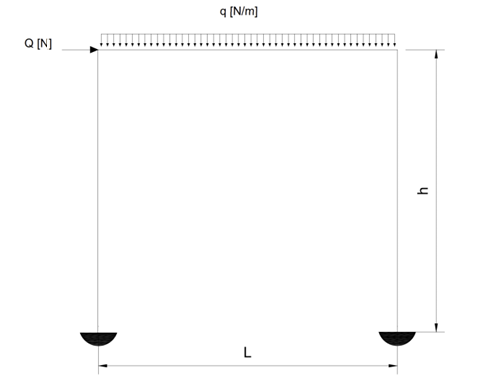
\includegraphics[width=0.65\textwidth]{problema.png}
    \caption{Estrutura a ser avaliada.}
    \label{fig: problema}
\end{figure}

\section{Métodos aplicados}

\subsection{Solução analítica}

Realizou-se a solução analítica através do método das forças, considerando o diagrama de corpo livre apresentado na figura~\ref{fig: dcl}, o qual resultou nas reações de apoio apresentadas na tabela~\ref{tab:reacoes analitico}.

\begin{figure}[H]
    \centering
    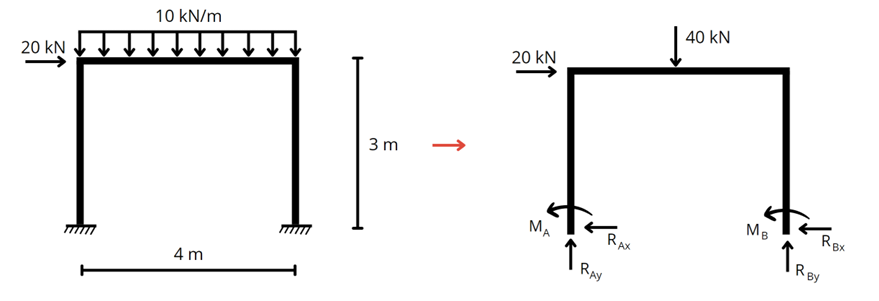
\includegraphics[width=1\textwidth]{dcl.png}
    \caption{Diagrama de corpo livre da estrutura avaliada.}
    \label{fig: dcl}
\end{figure}

\begin{table}[h!]
\centering
\caption{Reações de apoio obtidas através da solução analítica}

\renewcommand{\arraystretch}{1.3}

\begin{tabular}{c c c}
\hline
Reação & Apoio A & Apoio B \\ 
\hline
\hline
Momento [kNm]    & 12,91 & 22,57 \\
Vertical [kN]    & 13,87  & 26,13 \\
Horizontal [kN]  & 5,16 & 14,84 \\
\hline
\end{tabular}

\label{tab:reacoes analitico}
\end{table}

\subsection{Análise por elementos finitos}

A análise por elementos finitos teve início com a modelagem da estrutura no \textit{software} \textit{SolidWroks}, considerando as dimensões da seção transversal do perfil $W 200 x 15,0$ e as propriedades do aço ASTM A572 Grau 50. As simulações foram realizadas utilizando o \textit{software} \textit{Ansys 2023R2}, através do sistema de análise \textit{Static Structural}. As figuras~\ref{fig:portico_solid} e~\ref{fig:secao_w} apresentam a geometria modelada e seção transversal do perfil escolhido, enquanto a figura~\ref{fig: eng data} apresenta as propriedades do material inseridas no  \textit{Engineering data} do \textit{Workbench}. A tabela~\ref{tab: dimensoes perfil w} apresenta as dimensões do perfil escolhido. Uma vez que a geometria do modelo compreende apenas peças retas, optou-se pela simplificação utilizando elementos de casca.

\begin{figure}[H]
    \centering

    \begin{subfigure}[b]{0.46\textwidth}
        \centering
        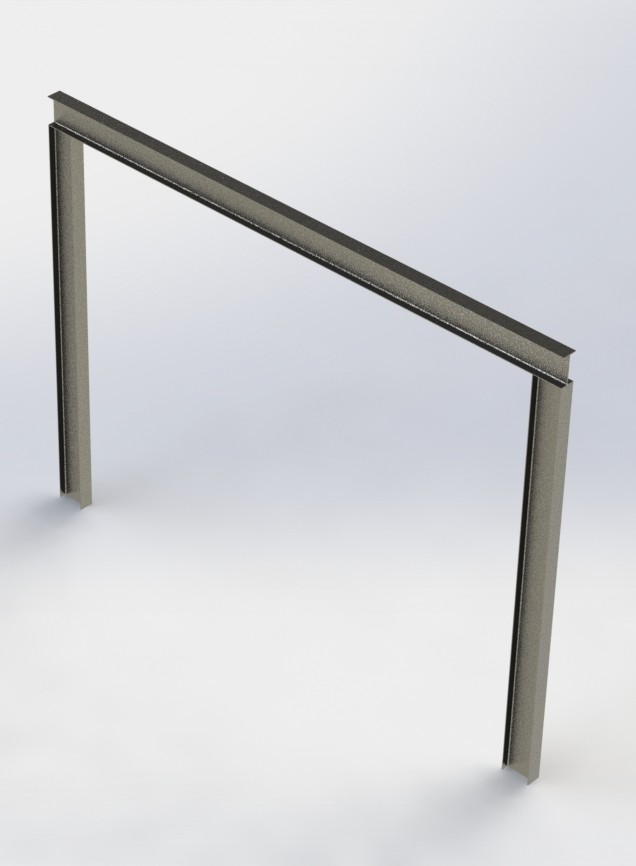
\includegraphics[width=\textwidth]{portico solid.JPG}
        \caption{Modelo no SolidWorks.}
        \label{fig:portico_solid}
    \end{subfigure}
    \hfill
    \begin{subfigure}[b]{0.48\textwidth}
        \centering
        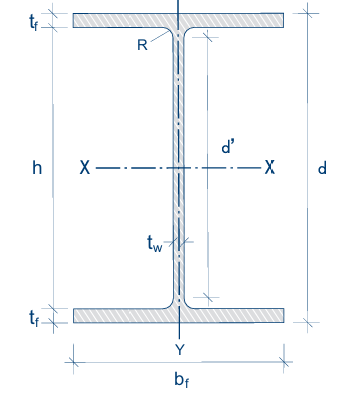
\includegraphics[width=\textwidth]{secao w.png}
        \caption{Seção transversal do perfil.}
        \label{fig:secao_w}
    \end{subfigure}

    \caption{Geometria e seção transversal da estrutura avaliada.}
    \label{fig:geometria_portico}
\end{figure}

\begin{table}[h!]
\centering
\caption{Dimensões do perfil W 200 x 15,0}

\renewcommand{\arraystretch}{1.3}

\begin{tabular}{c c c c c c c}
\hline
Dimensão & tf & h & d  & tw & bf & d' \\ 
\hline
Valor [mm] & 5,2 & 190 & 200 & 4,3 & 100 & 170  \\
\hline
\end{tabular}

\label{tab: dimensoes perfil w}
\end{table}

\begin{figure}[H]
    \centering
    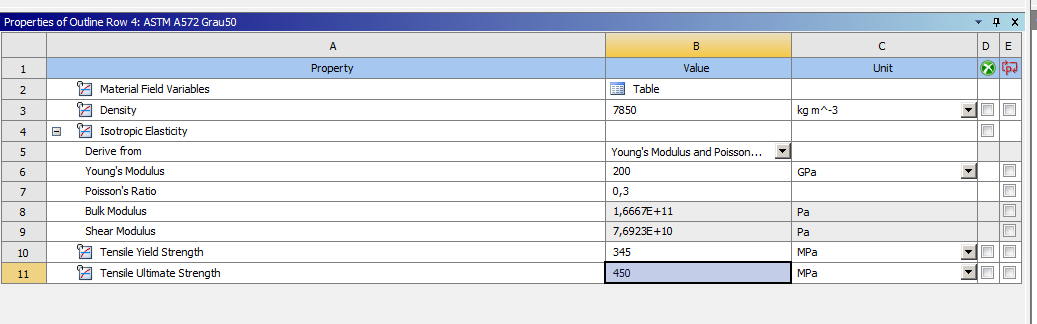
\includegraphics[width=1\textwidth]{prop aco.png}
    \caption{Propriedades do aço ASTM A572 Grau 50 utilizadas nas simulações.}
    \label{fig: eng data}
\end{figure}



Para a realização da simulação utilizando elementos de casca, realizou-se a importação e preparo da geometria no \textit{software Space Claim}, figura~\ref{fig:geom space 2d}, onde foram utilizados os recursos \textit{midsurface} e \textit{share topology}. 

\begin{figure}[H]
    \centering

    \begin{subfigure}[b]{0.48\textwidth}
        \centering
        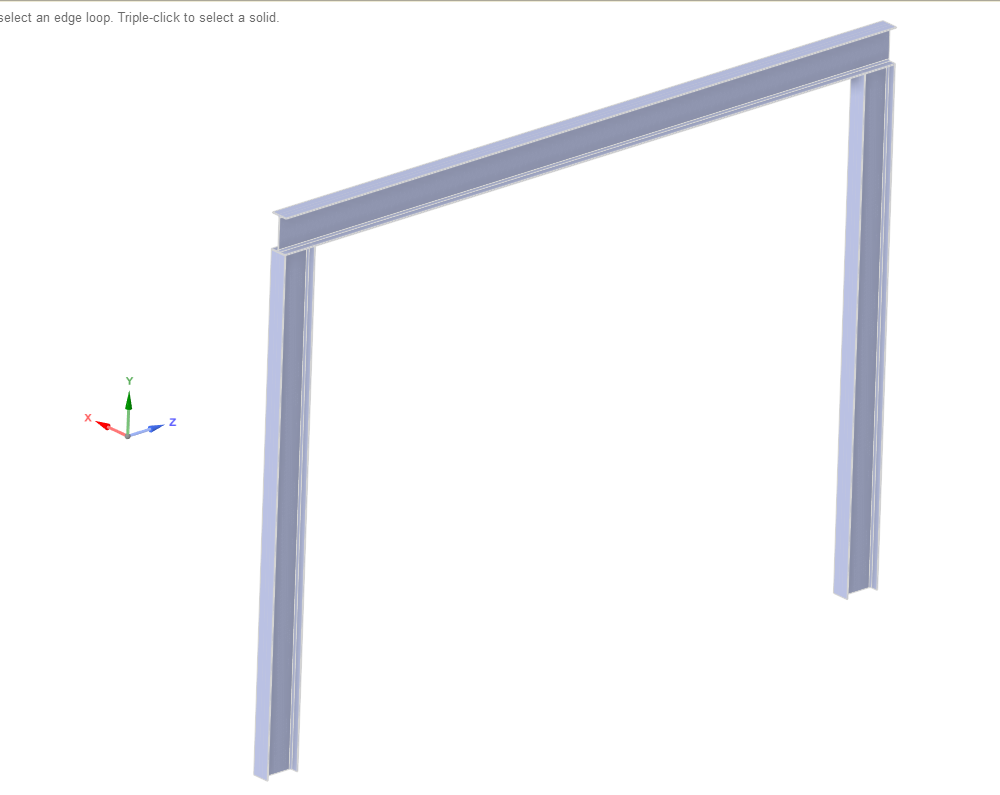
\includegraphics[width=\textwidth]{portico space shell.png}
        \caption{Modelo importado no Space Claim.}
        \label{fig:portico_solid}
    \end{subfigure}
    \hfill
    \begin{subfigure}[b]{0.48\textwidth}
        \centering
        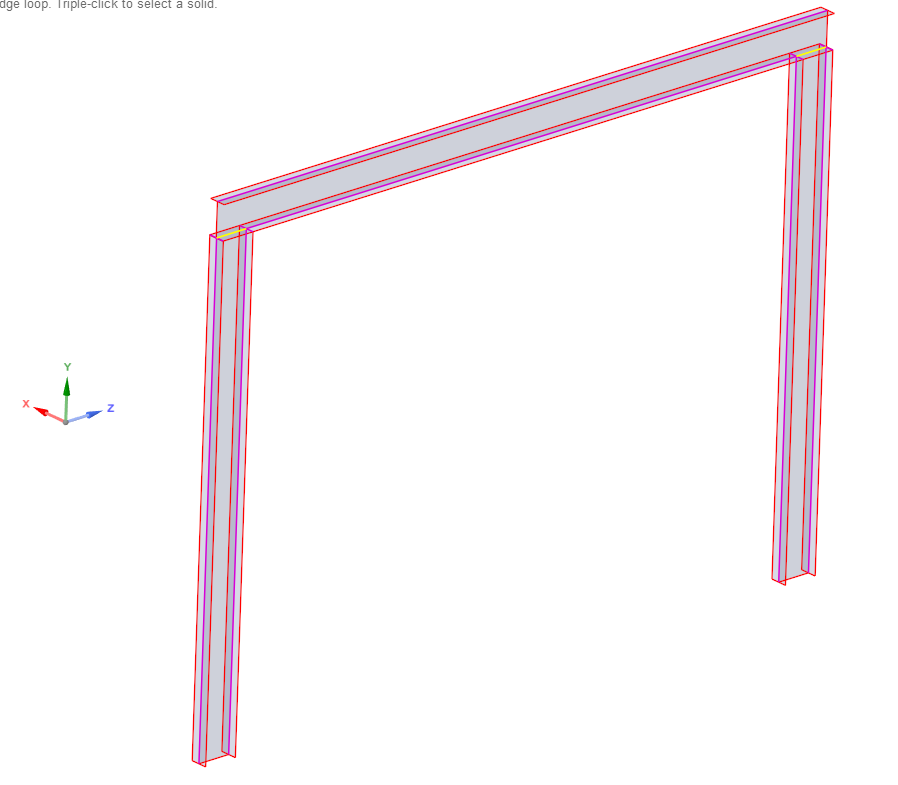
\includegraphics[width=\textwidth]{portico 2d.png}
        \caption{Modelo preparado para simulação.}
        \label{fig:secao_w}
    \end{subfigure}

    \caption{Modelo importado no Space Claim.}
    \label{fig:geom space 2d}
\end{figure}

Dentro do \textit{software Mechanical} foi gerada a malha com elementos triangulares de primeira ordem, utilizando inicialmente o tamanho padrão de elementos, 50 mm. Como critério de qualidade de malha foi monitorado o grau de distorção e assimetria dos elementos através do skewness. 

O estudo de convergência de malha foi realizado observando os valores das reações de apoio, os deslocamentos nas arestas da alma da viga sobre os pilares e a tensão máxima principal na aresta da alma da viga sobre a ligação com o pilar direito, representado na figura~\ref{fig: vertice monitorado}. O tamanho dos elementos foi variado de 50 a 10, adotando um refinamento local nas regiões de ligação viga-pilar, gerado através do recurso \textit{body sizing} do tipo \textit{sphere of influence}, considerando um raio de $500$~mm e com elementos com metade do tamanho do restante da malha, ilustrado na figura~\ref{fig: esfera}.

O carregamento distribuído na viga foi aplicado utilizando o recurso \textit{line pressure}, posicionando no centro da aba superior da viga. A força horizontal foi aplicada nas arestas da seção transversal da viga utilizando o recurso \textit{force}. A figura~\ref{fig: carregamentos} ilustra a aplicação dos carregamentos.


\begin{figure}[H]
    \centering

    \begin{subfigure}[b]{0.5\textwidth}
        \centering
        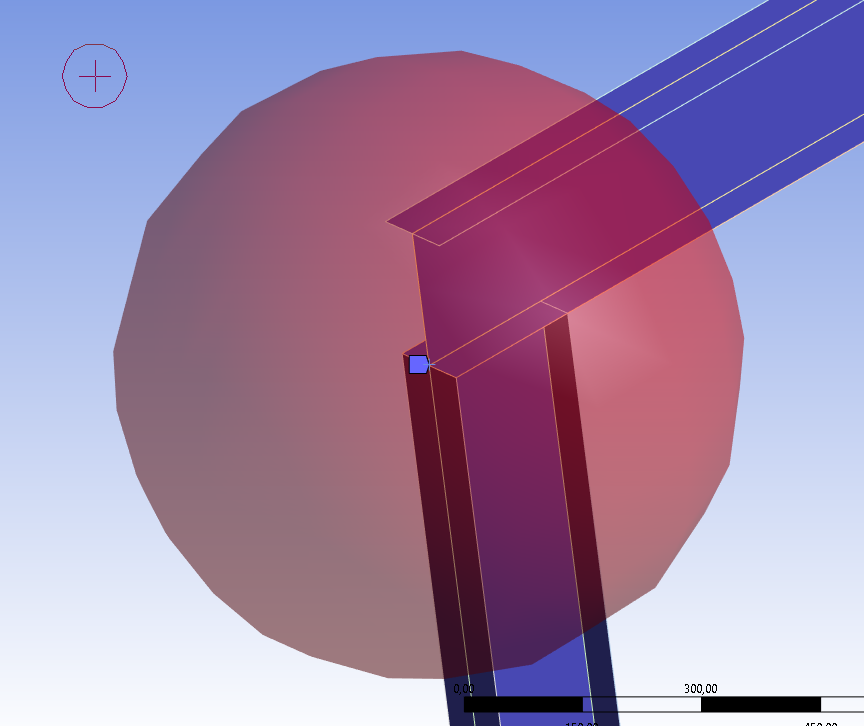
\includegraphics[width=\textwidth]{esfera .png}
        \caption{Esfera de influência.}
        \label{fig: esfera}
    \end{subfigure}
    \hfill
    \begin{subfigure}[b]{0.44\textwidth}
        \centering
        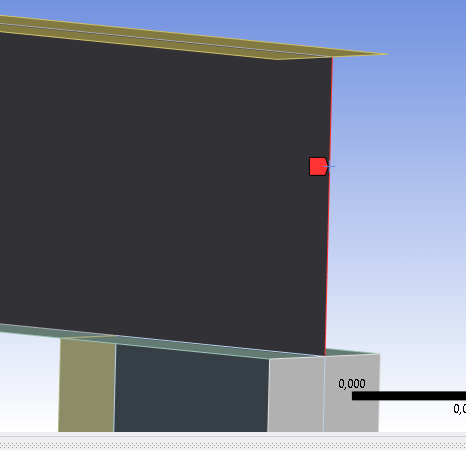
\includegraphics[width=\textwidth]{aresta alma.png}
        \caption{Vértice monitorado.}
        \label{fig: vertice monitorado}
    \end{subfigure}

    \caption{Modelo importado no Space Claim.}
    \label{fig:geom space 2d}
\end{figure}

\begin{figure}[H]
    \centering

    \begin{subfigure}[b]{0.5\textwidth}
        \centering
        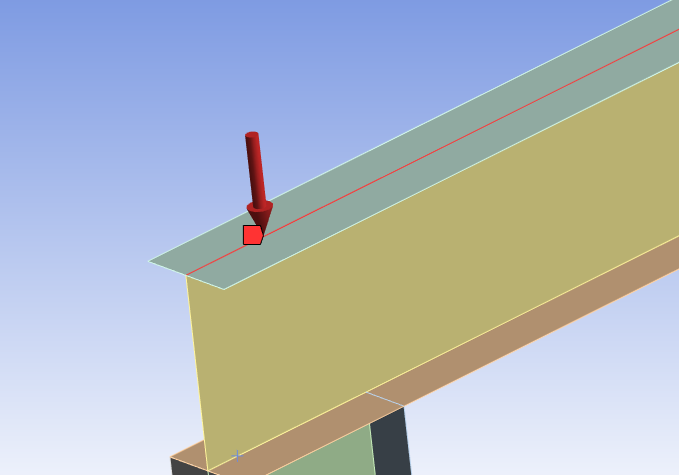
\includegraphics[width=\textwidth]{carga vertical.png}
        \caption{Carregamento vertical.}
        \label{fig:portico_solid}
    \end{subfigure}
    \hfill
    \begin{subfigure}[b]{0.46\textwidth}
        \centering
        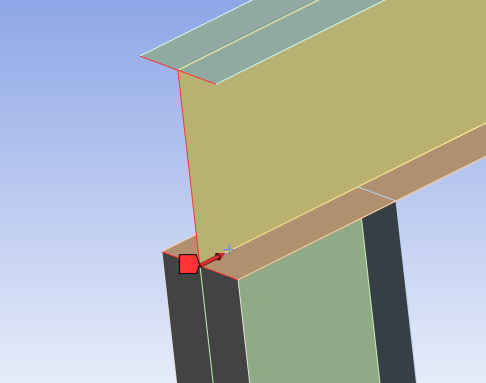
\includegraphics[width=\textwidth]{forca horizontal.png}
        \caption{Carregamento horizontal.}
        \label{fig:secao_w}
    \end{subfigure}

    \caption{Modelo importado no Space Claim.}
    \label{fig: carregamentos}
\end{figure}

\section{Resultados e discussão}

A análise de convergência realizada contou com malhas grosseiras e muito refinadas para a geometria em questão. A tabela~\ref{tab:estat malha} apresenta as estatísticas das malhas avaliadas. As malhas apresentaram um aumento no número de elementos de 26~\%, 42~\%, 59~\% e 72~\% quando comparadas com as imediatamente anteriores. Apesar do aumento significativo do número de elementos, o valor de de skewness médio e mínimo apresentou uma redução, enquanto o valor máximo apresentou uma flutuação entre $0,57$ e $0,77$, indicando que apesar do refinamento excessivo da malha, o critério de qualidade se manteve estável e com valor próximo a zero. Outro ponto a se ressaltar é que o valor máximo de $0,77$ foi observado em um elemento presente no meio do pilar direito, distante de aplicação de carregamentos, de modo a não influenciar significativamente no resultado das simulações.

\begin{table}[h!]
\centering
\caption{Estatísticas das malhas avaliadas}

\renewcommand{\arraystretch}{1.3}

\begin{tabular}{c c c c c c}
\hline
 & \multicolumn{5}{c}{Tamanho do elemento [mm]}\\
 
\hline
- & 50 & 40 & 30 & 20 & 10\\ 
\hline
\hline
Skewness máx.    & 0,57086 & 0,73871 & 0,67847 & 0,6504 & 0,77034 \\
Skewness min.    & 1,91E-06  & 4,59E-05 & 5,16E-06 & 7,0297E-06 & 5,9402E-07 \\
Skewness méd.    & 0,13373 & 0,15599 & 0,14707 & 0,12088 & 0,11366 \\
Número de elem.  & 4333 & 5887 & 10073 & 24403 & 87100 \\
Número de nós    & 2412 & 3250 & 5442 & 12805 & 44744 \\
\hline
\end{tabular}

\label{tab:estat malha}
\end{table}

A análise de convergência apresentou dois aspectos distintos, um em relação as reações de apoio e e outro entre as grandezas observadas nas seções transversais da viga. Os valores obtidos para as reações apresentaram rápida convergência, alcançando variações inferiores a 1~\% a partir da malha com elementos de 30~mm. Por outro lado, as deformações e tensões observadas continuaram variando, principalmente em seus valores máximos. 

Ao observar o local onde estes valores ocorriam, observou-se que o valor máximo era decorrente de uma singularidade na região de ligação entre a viga e o pilar direito, não representando de forma assertiva a física do problema. A tabela~\ref{tab:convergencia_malha} apresenta os valores monitorados durante o processo de convergência de malha, enquanto a tabela~\ref{tab:convergencia_diferencas} apresenta a diferença percentual entre os valores observados entre cada simulação, calculados com a equação ~\ref{eq:erro_percentual}, onde $X_{i}$ representa o resultado com a malha mais refinada e $X_{i-1}$ o resultado obtido com a malha anterior.

\begin{equation}
    \varepsilon_i =
    \left|
    \frac{X_{i-1} - X_i}{X_i}
    \right| \times 100\%
    \label{eq:erro_percentual}
\end{equation}



\begin{table}[H]
    \centering
    \caption{Resultados da análise de convergência de malha.}
    \label{tab:convergencia_malha}
    \small
    \renewcommand{\arraystretch}{1.2}
    \resizebox{\textwidth}{!}{%
    \begin{tabular}{l l c c c c c}
        \hline
        \multicolumn{2}{c}{} &
        \multicolumn{5}{c}{Tamanho do elemento [mm]} \\
        \cline{3-7}
        Unidade & Variável & 50 & 40 & 30 & 20 & 10 \\
        \hline
        N & $R_{Ax}$ & 6101,1 & 6029,9 & 6018,3 & 6021,5 & 6020,9 \\
        N & $R_{Ay}$ & 14394 & 14312 & 14341 & 14298 & 14297 \\
        N$\cdot$m & $M_A$ & 14630 & 14393 & 14455 & 14376 & 14375 \\
        N & $R_{Bx}$ & 13899 & 13970 & 13982 & 13978 & 13979 \\
        N & $R_{By}$ & 25606 & 25688 & 25659 & 25702 & 25703 \\
        N$\cdot$m & $M_B$ & 22035 & 21961 & 22012 & 21924 & 21920 \\
        \hline
        mm & Deslocamento seção esquerda (máx.)
           & 13,979 & 14,554 & 14,629 & 14,981 & 14,115 \\
        mm & Deslocamento seção esquerda (méd.)
           & 13,439 & 13,991 & 14,061 & 14,402 & 14,517 \\
        mm & Deslocamento seção esquerda (mín.)
           & 12,893 & 13,422 & 13,487 & 13,817 & 13,942 \\
        mm & Deslocamento seção direita (máx.)
           & 13,348 & 13,901 & 13,972 & 14,314 & 14,444 \\
        mm & Deslocamento seção direita (méd.)
           & 13,302 & 13,853 & 13,921 & 14,262 & 14,392 \\
        mm & Deslocamento seção direita (mín.)
           & 13,238 & 13,785 & 13,852 & 14,191 & 14,318 \\
        \hline
        MPa & Tensão principal na alma direita (máx.)
            & 543,18 & 651,37 & 675,19 & 760,5 & 1311,8 \\
        MPa & Tensão principal na alma direita (méd.)
            & 243,5 & 254,97 & 255,09 & 265,48 & 282,42 \\
        MPa & Tensão principal na alma direita (mín.)
            & 29,607 & 22,313 & 16,226 & 11,519 & 4,8915 \\
        \hline
        MPa & Tensão equivalente de von Mises (máx.)
            & 551,33 & 630,4 & 652,13 & 740,07 & 1240,2 \\
        MPa & Tensão equivalente de von Mises (méd.)
            & 58,773 & 61,778 & 61,76 & 62,474 & 62,127 \\
        MPa & Tensão equivalente de von Mises (mín.)
            & 0,12575 & 0,083277 & 0,094177 & 0,038077 & 0,068529 \\
        \hline
        mm & Deslocamento total (máx.)
           & 14,461 & 15,06 & 15,154 & 15,509 & 15,648 \\
        mm & Deslocamento total (méd.)
           & 10,628 & 11,114 & 11,599 & 11,923 & 12,317 \\
        mm & Deslocamento total (mín.)
           & 0 & 0 & 0 & 0 & 0 \\
        \hline
    \end{tabular}%
    }
\end{table}

Ao comparar o resultado das reações obtidos com as simulações com os calculados através do método analítico observou-se a maior diferença na reação horizontal na base do pilar esquerdo, com valor de 16,68~\%, e a de menor diferença na reação vertical na base do pilar direito, com 1,63~\%. Apesar da diferença considerada alta, a mesma foi atribuída as simplificações realizadas durante o calculo analítico, entre elas a desconsideração dos esforços cortantes e normais.

Uma vez que os resultados obtidos apresentaram valores médios com discrepância majoritariamente inferior a 3~\%, com os valores máximos sendo observados no mesmo ponto e que seguem aumentando conforme o refinamento da malha, considerou-se o comportamento observado como o de uma singularidade de tensão decorrente da idealização da conexão entre a viga e o pilar. Deste modo, os valores máximos locais não foram considerados representativos para a avaliação da estrutura, permanecendo registrados como uma limitação do recurso numérico.

\begin{table}[H]
    \centering
    \caption{Diferenças percentuais entre refinamentos sucessivos da malha.}
    \label{tab:convergencia_diferencas}
    \small
    \renewcommand{\arraystretch}{1.2}
    \resizebox{\textwidth}{!}{%
    \begin{tabular}{l c c c c c}
        \hline
        & \multicolumn{5}{c}{Tamanho do elemento [mm]} \\
        \cline{2-6}
        Variável & 50 & 40 & 30 & 20 & 10 \\
        \hline
        $R_{Ax}$ & -- & 1,18\% & 0,19\% & 0,05\% & 0,01\% \\
        $R_{Ay}$ & -- & 0,57\% & 0,20\% & 0,30\% & 0,01\% \\
        $M_A$    & -- & 1,65\% & 0,43\% & 0,55\% & 0,01\% \\
        $R_{Bx}$ & -- & 0,51\% & 0,09\% & 0,03\% & 0,01\% \\
        $R_{By}$ & -- & 0,32\% & 0,11\% & 0,17\% & 0,00\% \\
        $M_B$    & -- & 0,34\% & 0,23\% & 0,40\% & 0,02\% \\
        \hline
        Deslocamento seção esquerda (máx.)
        & -- & 3,95\% & 0,51\% & 2,35\% & 6,14\% \\
        Deslocamento seção esquerda (méd.)
        & -- & 3,95\% & 0,50\% & 2,37\% & 0,79\% \\
        Deslocamento seção esquerda (mín.)
        & -- & 3,94\% & 0,48\% & 2,39\% & 0,90\% \\
        Deslocamento seção direita (máx.)
        & -- & 3,98\% & 0,51\% & 2,39\% & 0,90\% \\
        Deslocamento seção direita (méd.)
        & -- & 3,98\% & 0,49\% & 2,39\% & 0,90\% \\
        Deslocamento seção direita (mín.)
        & -- & 3,97\% & 0,48\% & 2,39\% & 0,89\% \\
        \hline
        Tensão principal na alma direita (máx.)
        & -- & 16,61\% & 3,53\% & 11,22\% & 42,03\% \\
        Tensão principal na alma direita (méd.)
        & -- & 4,50\% & 0,05\% & 3,91\% & 6,00\% \\
        Tensão principal na alma direita (mín.)
        & -- & 32,69\% & 37,51\% & 40,86\% & 135,49\% \\
        \hline
        Tensão equivalente de von Mises (máx.)
        & -- & 12,54\% & 3,33\% & 11,88\% & 40,33\% \\
        Tensão equivalente de von Mises (méd.)
        & -- & 4,86\% & 0,03\% & 1,14\% & 0,56\% \\
        Tensão equivalente de von Mises (mín.)
        & -- & 51,00\% & 11,57\% & 147,33\% & 44,44\% \\
        \hline
        Deslocamento total (máx.)
        & -- & 3,98\% & 0,62\% & 2,29\% & 0,89\% \\
        Deslocamento total (méd.)
        & -- & 4,37\% & 4,18\% & 2,72\% & 3,20\% \\
        \hline
    \end{tabular}%
    }
\end{table}

Ao analisar os resultados da tensão equivalente de von-Mises próximo a singularidade, figura~\ref{fig: dist local}, observa-se que a tensão na região é inferior ao limite de escoamento do aço ASTM A572 Grau 50 (345 MPa). Além disso, ao avaliar os valores de tensão por toda a estrutura, figura~\ref{fig: dist geral}, observa-se que ao longo da estrutura o valor obtido é inferior a 10~\% do limite ao escoamento. 

Por fim, ao observar o deslocamento total da estrutura, observou-se valores máximo de 15,65~mm, os quais foram considerados irrisórios, uma vez que representam 0,39~\% quando comparado ao vão do pórtico. A figura~\ref{fig: def total} apresenta a deformação total sofrida pela estrutura.  

\begin{figure}[H]
    \centering
    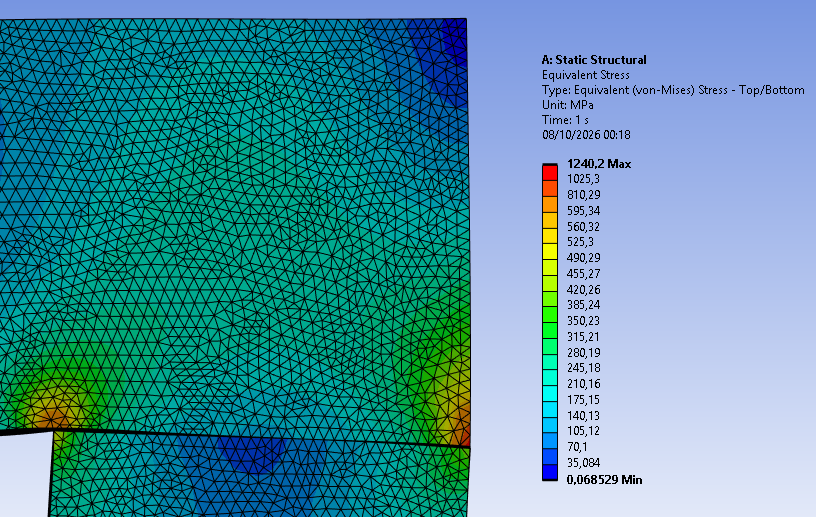
\includegraphics[width=1\textwidth]{distribuicao de tensao local.png}
    \caption{Distribuição de tensão próximo a singularidade.}
    \label{fig: dist local}
\end{figure}

\begin{figure}[H]
    \centering
    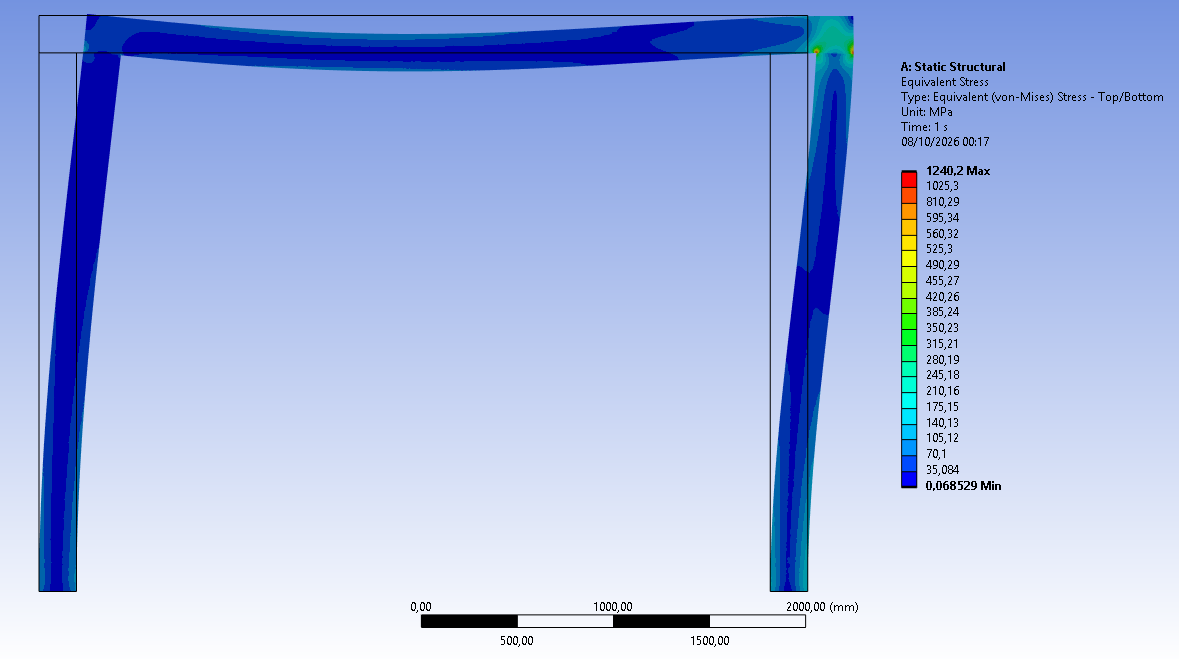
\includegraphics[width=1\textwidth]{distribuicao de tensao geral.png}
    \caption{Distribuição de tensão ao longo do modelo.}
    \label{fig: dist geral}
\end{figure}

\begin{figure}[H]
    \centering
    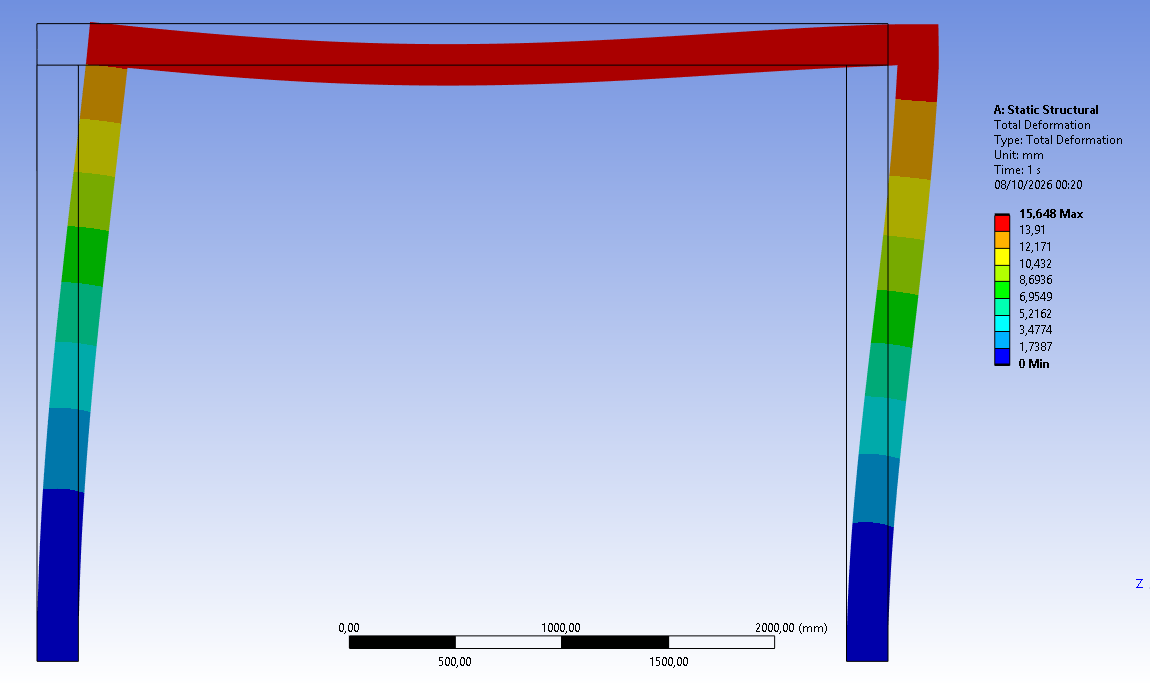
\includegraphics[width=1\textwidth]{deformacao total.png}
    \caption{Deformação total do modelo.}
    \label{fig: def total}
\end{figure}

\section{Conclusão}

O presente trabalho permitiu aplicar os conceitos fundamentais do Método dos Elementos Finitos à análise estrutural de um pórtico hiperestático, por meio da comparação entre uma solução analítica, obtida pelo método das forças, e uma solução numérica desenvolvida no ANSYS Mechanical. A utilização de elementos de casca possibilitou representar a geometria dos perfis metálicos e avaliar a distribuição de deslocamentos e tensões na estrutura, além de investigar a influência da qualidade e do grau do refinamento da malha sobre os resultados obtidos.

A comparação entre as reações de apoio calculadas analiticamente e aquelas obtidas numericamente demonstrou diferenças percentuais entre 1,63~\% e 16,68~\%, sendo a maior discrepância observada na reação horizontal do apoio esquerdo. Essas diferenças podem estar relacionadas às simplificações adotadas na formulação analítica, especialmente à desconsideração das deformações associadas aos esforços normais e cortantes.

O estudo de convergência de malha, realizado com tamanhos de elementos entre 50 e 10 mm, demonstrou a estabilização das reações de apoio, com diferenças inferiores a 0,02~\% entre as malhas de 20 e 10 mm. Os deslocamentos globais também apresentaram tendência de convergência, com diferença de 0,89~\% para o deslocamento máximo entre os dois últimos refinamentos. Para a malha mais refinada, o deslocamento máximo foi de 15,65 mm, correspondente a aproximadamente 0,39~\% do vão de 4 m.

Por outro lado, as tensões máximas apresentaram comportamento distinto, aumentando progressivamente com o refinamento da malha. A tensão equivalente máxima de von Mises passou de 551,33 MPa para 1240,2 MPa, enquanto os valores médios globais permaneceram relativamente estáveis. A análise da distribuição espacial das tensões evidenciou concentrações localizadas nas regiões de ligação entre a viga e o pilar direito, comportamento compatível com a presença de singularidades de tensão associadas à idealização geométrica dessa conexão. Deste modo, os valores máximos locais foram mantidos nos resultados, mas sua utilização direta para a verificação da resistência estrutural requer uma investigação adicional.

Conclui-se que a discretização adotada foi suficiente para demonstrar a convergência das reações de apoio e a tendência de estabilização dos deslocamentos globais e da média da tensão equivalente de von-Mises. Também é possível concluir que a estrutura proposta cumpre com o critério estabelecido no objetivo do presente trabalho, uma vez que a distribuição de tensão apresenta majoritariamente, com exceção da singularidade, valores inferiores a tensão limite de escoamento.

Por fim, a análise desenvolvida contribuiu para a compreensão das etapas de preparação geométrica, definição das condições de contorno, geração e avaliação da qualidade da malha e interpretação dos resultados obtidos pelo Método dos Elementos Finitos. 

\printbibliography[heading=bibintoc,title={Referências}]



\end{document}